\documentclass[10pt,pdf]{beamer}
\mode<presentation>
\usetheme{Warsaw}
\usecolortheme{whale}

% \usepackage[utf8]{inputenc}
% \usepackage[T2A]{fontenc}
% \usepackage[russian,english]{babel}

\usepackage{amssymb}
\usepackage{amsmath}
\usepackage{graphicx}
\usepackage{epstopdf}
\usepackage[english]{isodate}
\usepackage[noend]{algorithmic}
\usepackage{algorithm}
\usepackage{multirow}
\usepackage{tikz}
\usepackage{pgfplots}
\usepackage{tabulary}

\algsetup{indent=2em,linenosize=\footnotesize}

\title{Automatic Mobile Video Director}
\author{
	{Alexander Egurnov}
	{University of Mannheim\\
		aegurnov@mail.uni-mannheim.de}
\and \\
	{Thilo Weigold}
	{University of Mannheim\\
		tweigold@mail.uni-mannheim.de}
\and \\
	{Jon Pettersen}
	{University of Oslo\\
		jonup@student.matnat.uio.no}
\and \\
	{Alf-André Walla}
	{University of Oslo\\
		alfandrw@ifi.uio.no}
}
\institute[University of Mannheim]{University of Mannheim}

\begin{document}

% \AtBeginSection[]
% {
%     \begin{frame}
%         \frametitle{Table of Contents}
%         \tableofcontents[currentsection]
%     \end{frame}
% }

% \AtBeginSubsection[]
% {
%     \begin{frame}
%         \frametitle{Table of Contents}
%         \tableofcontents[currentsection, currentsubsection]
%     \end{frame}
% }
\setcounter{framenumber}{0}
\setbeamertemplate{footline}
{
  \leavevmode%
  \hbox{%
  %\begin{beamercolorbox}[wd=.333333\paperwidth,ht=2.25ex,dp=1ex,center]{author in head/foot}%
	%\usebeamerfont{author in head/foot}\insertshortauthor%~~\beamer@ifempty{\insertshortinstitute}{}{(\insertshortinstitute)}
  %\end{beamercolorbox}%
  \begin{beamercolorbox}[wd=.4\paperwidth,ht=2.25ex,dp=1ex,center]{title in head/foot}%
	\usebeamerfont{title in head/foot}\insertshorttitle
  \end{beamercolorbox}%
  \begin{beamercolorbox}[wd=.4\paperwidth,ht=2.25ex,dp=1ex,center]{institute in head/foot}%
	\usebeamerfont{institute in head/foot}\insertinstitute
  \end{beamercolorbox}%
  \begin{beamercolorbox}[wd=.2\paperwidth,ht=2.25ex,dp=1ex,right]{date in head/foot}%
	\insertframenumber{} / \inserttotalframenumber\hspace*{2ex} 
  \end{beamercolorbox}}%
  \vskip0pt%
}

\begin{frame}
	\titlepage
\end{frame}

\begin{frame}
	\frametitle{Contents}
	\tableofcontents
\end{frame}

\section{Section 1}

\subsection{Subsection} 
\begin{frame}
	\frametitle{Frame 1}
	\begin{itemize}
		\item One
		\item Two
		\item Three
	\end{itemize}
\end{frame}

\begin{frame}
	\frametitle{Frame 2}
	\begin{itemize}
		\item Four
		\item Five
	\end{itemize}
\end{frame}

\section{Section 2}
\begin{frame}
	\frametitle{Two Columns}
	\begin{columns}[t]
		\begin{column}[c]{5cm}
			\footnotesize
			\begin{tabular}[H]{|l||c|c|c|c|}
		        \hline
		        & \rotatebox{90}{Sugar } & \rotatebox{90}{Juicy } & \rotatebox{90}{Healthy } & \rotatebox{90}{Natural } \\
		        \hline
		        Fruit chews & $\times$ & $\times$ & & \\
		        \hline
		        Lollipop & $\times$ & & & \\
		        \hline
		        Chewing gum & & & $\times$ & \\
		        \hline
		        Fresh fruit & & $\times$ & $\times$ & $\times$ \\
		        \hline
		    \end{tabular}
		\end{column}
		\begin{column}[c]{5cm}
			\usetikzlibrary{shapes.geometric}
			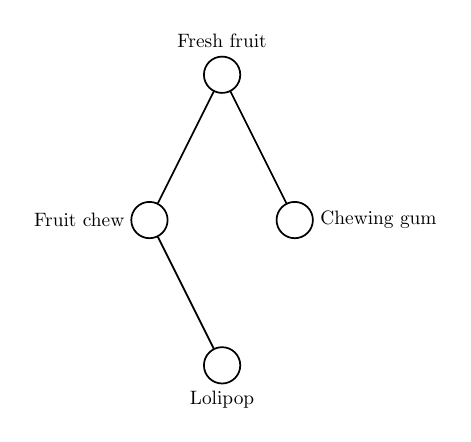
\begin{tikzpicture}[thick,scale=0.7, every node/.style={transform shape}]
				% [every node/.style={inner sep=0pt}]
				\node (1) [circle, minimum size=18.75pt, fill=white, line width=0.625pt, draw=black] at (187.5pt, -75.0pt)  {};
				\node (4) [circle, minimum size=18.75pt, fill=white, line width=0.625pt, draw=black] at (187.5pt, -225.0pt)  {};
				\node (2) [circle, minimum size=18.75pt, fill=white, line width=0.625pt, draw=black] at (150.0pt, -150.0pt)  {};
				\node (3) [circle, minimum size=18.75pt, fill=white, line width=0.625pt, draw=black] at (225.0pt, -150.0pt)  {};
				\draw [line width=0.625, color=black] (2) to  (1);
				\draw [line width=0.625, color=black] (3) to  (1);
				\draw [line width=0.625, color=black] (4) to  (2);
				\node at (187.5pt, -57.5pt) {\textcolor{black}{Fresh fruit}};
				\node at (187.5pt, -242.5pt) {\textcolor{black}{Lolipop}};
				\node at (113.75pt, -150.0pt) {\textcolor{black}{Fruit chew}};
				\node at (268.25pt, -150.0pt) {\textcolor{black}{Chewing gum}};
			\end{tikzpicture}
		\end{column}
	\end{columns}
\end{frame}

\end{document}
